\documentclass[11pt,aspectratio=169,handout]{beamer}
\providecommand{\scseries}{\scshape}
\usepackage{paislidestempo}
\setlength{\parskip}{0.45em}
\setbeamertemplate{itemize/enumerate body begin}{\vspace{-0.5em}}
\def\meditem{\smallskip\item}
\setbeamerfont{normal text}{size=\small}
\AtBeginDocument{\usebeamerfont{normal text}}
\setbeamerfont{block title}{size=\small}
\setbeamerfont{frametitle}{size=\large}
\setbeamersize{text margin left=7mm,text margin right=7mm}
\usepackage{amsmath,amssymb,booktabs}
\usepackage{pgfplots}
\pgfplotsset{compat=1.18}
\usetikzlibrary{positioning,decorations.pathreplacing,calc,fit,patterns}

\newcommand{\SPA}{\mathrm{SPA}}
\newcommand{\uq}{\underline q}
\newcommand{\oq}{\bar q}
\newcommand{\tsc}[1]{\textsc{#1}}
\newcommand{\good}[1]{{\color{PosDark}#1}}
\newcommand{\bad}[1]{{\color{NegDark}#1}}

% picture colours: the deviator is ink, the rivals are grey, a pool is orange
\colorlet{Dev}{Ink}
\colorlet{Riv}{Line}
\colorlet{Pool}{Warn}
\tikzset{
  ax/.style={-{Stealth[length=1.8mm]},InkTwo,line width=0.5pt},
  lab/.style={font=\footnotesize},
  slab/.style={font=\scriptsize,text=InkTwo},
  box/.style={draw=Line,rounded corners=2pt,fill=Card,align=center,font=\footnotesize,inner sep=4pt},
  hl/.style={draw=Ink,rounded corners=2pt,fill=Ink,text=white,align=center,font=\footnotesize,inner sep=4pt},
  br/.style={decorate,decoration={brace,amplitude=3pt},InkTwo},
  brm/.style={decorate,decoration={brace,amplitude=3pt,mirror},InkTwo},
  curve/.style={line width=1pt,Ink},
  dev/.style={line width=1.3pt,Pool},
}
\pgfplotsset{every axis/.append style={axis line style={InkTwo},tick style={InkTwo},
  tick label style={font=\scriptsize},label style={font=\footnotesize},
  legend style={fill=none,draw=none,font=\scriptsize}}}

% a segment of the type line: \seg{x0}{x1}{fill}{y}
\def\seg#1#2#3#4{\fill[#3,draw=InkTwo,line width=0.3pt] (#1,#4) rectangle (#2,#4+0.42);}

% one panel of a quantity path: #1 title, #2 the path, #3 caption
\newcommand{\pathpanel}[3]{%
\begin{tikzpicture}[scale=1.34]
  \draw[ax] (0,0)--(1.12,0) node[below,slab]{$q$};
  \draw[ax] (0,0)--(0,1.12) node[left,slab]{$t$};
  \draw[Line,dashed] (0,0)--(1,1);
  #2
  \node[font=\scriptsize\scshape,anchor=south] at (0.55,1.13) {#1};
  \node[slab,anchor=north] at (0.55,-0.12) {#3};
\end{tikzpicture}}

\begin{document}

\title[Auction Design under Competition]{Auction Design under Competition}
\author[Mallesh Pai]{\large\textsc{Mallesh M. Pai}}
\institute[Tempo]{\vspace{4mm}\inserttitlegraphic}
\date{\textsc{November 2026}}

\begin{frame}
\maketitle
\end{frame}

%%%%%%%%%%%%%%%%%%%%%%%%%%%%%%%%%%%%%%%%%%%%%%%%%%%%%%%%%%%%%%%%%%%%
\section{Motivation}
%%%%%%%%%%%%%%%%%%%%%%%%%%%%%%%%%%%%%%%%%%%%%%%%%%%%%%%%%%%%%%%%%%%%

\begin{frame}{Two Distortions in Monopoly (Myerson 1981, Bulow \& Roberts 1989)}
A monopolist facing i.i.d.\ buyers from $F$ acts like a price-setter facing demand $P(z)=F^{-1}(1-z)$ with marginal revenue $\psi_1(v)=v-\frac{1-F(v)}{f(v)}$. Two distinct inefficiencies can arise:

\medskip
\begin{columns}[T]
\begin{column}{0.47\textwidth}
1. \alert{Withholding}: refuses to sell below a reserve price even when $v > \text{cost}$.

\bigskip
\centering
\begin{tikzpicture}[xscale=6.4]
  \seg{0}{0.3}{Tint}{0}\seg{0.3}{1}{Card}{0}
  \node[slab] at (0.15,0.21) {excluded};\node[slab] at (0.65,0.21) {efficient auction};
  \node[lab,below] at (0.3,-0.02) {reserve};
  \node[slab,below] at (0.04,-0.02) {low $v$};\node[slab,below] at (0.95,-0.02) {high $v$};
\end{tikzpicture}
\end{column}
\begin{column}{0.47\textwidth}
2. \alert{Misallocation}: \alert{pools} an interval of types and rations randomly, so a lower value can beat a higher one.

\bigskip
\centering
\begin{tikzpicture}[xscale=6.4]
  \seg{0}{0.3}{Tint}{0}\seg{0.3}{0.46}{Card}{0}\seg{0.46}{0.82}{Pool!55}{0}\seg{0.82}{1}{Card}{0}
  \node[slab] at (0.15,0.21) {excluded};\node[slab] at (0.64,0.21) {treated alike};
  \node[lab,below] at (0.3,-0.02) {reserve};
  \node[lab,below,text=Pool] at (0.64,-0.02) {a pool};
\end{tikzpicture}
\end{column}
\end{columns}

\bigskip\onslide<2->
\begin{block}{Myerson (1981)}
A monopolist withholds when $\psi_1 < 0$, and misallocates (irons) when $\psi_1$ is not increasing. A second price auction with a reserve may withhold, but never misallocates.
\end{block}
\end{frame}

\begin{frame}{What Should We Expect in an Oligopoly?}
\begin{itemize}
\item \alert{Monopoly} (Myerson 1981): withholding, and misallocation unless $\psi_1$ is increasing (regularity).
\meditem \alert{Perfect competition} (McAfee 1993, Peters \& Severinov 1997): both inefficiencies vanish---every seller posts a second price auction with reserve equal to cost.
\meditem \alert{Finite oligopoly}: existing literature forces sellers to use second price auctions and studies competition in reserves (Burguet \& S\'akovics 1999, Vir\'ag 2010). Speaks to withholding, but \emph{assumes misallocation away}.
\end{itemize}

\medskip\onslide<2->
\begin{block}{This paper}
$m$ sellers with one unit each, $n$ buyers. Each seller chooses \emph{how} to sell (a reserve and any pooling intervals). When does competition eliminate misallocation, when does it create new motives to misallocate, and what replaces Myerson's regularity?
\end{block}
\end{frame}

\begin{frame}{Covered Markets vs.\ Binding Reserves}
Sellers' cost is $0$. One question splits the analysis: does a reserve price exclude any buyers?

\medskip
\begin{columns}[T]
\begin{column}{0.47\textwidth}
\centering
\alert{Covered market} ($a>0$, $\rho<a$)

\smallskip
\begin{tikzpicture}[xscale=5.3,yscale=1.85]
  \fill[Tint] plot[smooth] coordinates {(0.42,0.5) (0.58,0.95) (0.78,0.8) (1,0.42)} -- (1,0) -- (0.42,0) -- cycle;
  \draw[curve] (0.42,0)--(0.42,0.5) plot[smooth] coordinates {(0.42,0.5) (0.58,0.95) (0.78,0.8) (1,0.42)} (1,0.42)--(1,0);
  \draw[ax] (0,0)--(1.1,0) node[right,slab]{$v$};
  \path (0,0) rectangle (1.1,1.35);
  \draw[dev] (0.2,0)--(0.2,1.1);
  \node[slab,text=Pool,above] at (0.2,1.1) {reserve};
  \node[slab] at (0.72,0.35) {buyers' values};
  \node[lab,below] at (0,0) {cost};\node[lab,below] at (0.42,0) {$a$};\node[lab,below] at (1,0) {$1$};
\end{tikzpicture}

\raggedright\smallskip
Every buyer values the good strictly above cost. Reserve excludes nobody; it only prices a lone visitor.
\end{column}
\begin{column}{0.47\textwidth}
\onslide<2->
\centering
\alert{Binding reserve} ($\rho\ge a$)

\smallskip
\begin{tikzpicture}[xscale=5.3,yscale=1.85]
  \fill[Tint] plot[smooth] coordinates {(0,0.45) (0.3,0.95) (0.62,0.8) (1,0.42)} -- (1,0) -- (0,0) -- cycle;
  \begin{scope}\clip (0,0) rectangle (0.3,1.3);
  \fill[Neg,opacity=0.35] plot[smooth] coordinates {(0,0.45) (0.3,0.95) (0.62,0.8) (1,0.42)} -- (1,0) -- (0,0) -- cycle;\end{scope}
  \draw[curve] (0,0)--(0,0.45) plot[smooth] coordinates {(0,0.45) (0.3,0.95) (0.62,0.8) (1,0.42)} (1,0.42)--(1,0);
  \draw[ax] (0,0)--(1.1,0) node[right,slab]{$v$};
  \path (0,0) rectangle (1.1,1.35);
  \draw[dev] (0.3,0)--(0.3,1.1);
  \node[slab,text=Pool,above] at (0.3,1.1) {reserve};
  \node[slab,text=NegDark] at (0.15,0.25) {excluded};
  \node[lab,below] at (0,0) {cost};\node[lab,below] at (1,0) {$1$};\node[lab,below] at (0.42,0) {\phantom{$a$}};
\end{tikzpicture}

\raggedright\smallskip
Low-value buyers are excluded, and buyers just above the reserve earn virtually zero surplus at every seller.
\end{column}
\end{columns}
\end{frame}

\begin{frame}{Roadmap of Results}
A competing auctioneer's revenue is a weighted integral of \alert{Cournot oligopoly revenues} over market price levels, so Cournot's marginal revenue
\[
\psi_m(v) \;=\; v - \frac{1}{m}\,\frac{1-F(v)}{f(v)}
\]
replaces Myerson's virtual value (interpolating from Myerson $m=1$ to McAfee $m\to\infty$).

\medskip\onslide<2->
\begin{enumerate}
\item \alert{Covered markets}: if $\psi_m$ is nondecreasing and $\psi_m(a)\ge 0$, symmetric second price auctions survive \emph{all} pooling and reserve deviations, for every $n\ge 2$.
\meditem \alert{Binding reserves}: competition creates a new motive to misallocate---symmetric standard auctions always fail via an \emph{asking price}, and for large $n$ asymmetric duopoly profiles with $\psi_1(r_H)<0$ also fail against a pool.
\meditem \alert{Sharpness}: Cournot's curvature bound $E\le m+1$ is tight across $n$, while for narrow pools at any fixed $n$ the exact markup weight is $\varpi(m)=\frac{m+1}{m^2+2m-1}<\frac1m$.
\end{enumerate}
\end{frame}

%%%%%%%%%%%%%%%%%%%%%%%%%%%%%%%%%%%%%%%%%%%%%%%%%%%%%%%%%%%%%%%%%%%%
\section{Model}
%%%%%%%%%%%%%%%%%%%%%%%%%%%%%%%%%%%%%%%%%%%%%%%%%%%%%%%%%%%%%%%%%%%%

\begin{frame}{Model}
\begin{itemize}
\item $m\ge 2$ sellers, each with $1$ unit of an identical good (cost $0$).
\item $n\ge 2$ buyers with unit demand, values i.i.d.\ from $F$ on $[a,1]$ with continuous positive density $f$.
\item Market is \emph{covered} if $a>0$.
\end{itemize}

\bigskip
\centering
\begin{tikzpicture}[node distance=7mm]
  \node[box,text width=3.6cm] (a) {\textsc{1. Sellers}\\simultaneously announce mechanisms};
  \node[box,text width=3.6cm,right=of a] (b) {\textsc{2. Buyers}\\learn their values, see all mechanisms, and visit one seller};
  \node[box,text width=3.6cm,right=of b] (c) {\textsc{3. Trade}\\each seller runs his mechanism among his visitors};
  \draw[ax] (a)--(b); \draw[ax] (b)--(c);
\end{tikzpicture}

\raggedright\bigskip
We study weak perfect Bayesian equilibrium in anonymous mechanisms and buyer-symmetric visit strategies.
\end{frame}

\begin{frame}{Hierarchical Mechanisms}
A seller announces $\mathbf{m}=(r,\mathcal P)$: a reserve $r\in[0,1]$ and a finite collection $\mathcal P$ of disjoint pooling intervals in $(r,1)$.
\begin{itemize}
\item Types below $r$ are excluded; types in a common pool are tied (broken uniformly at random); otherwise higher reports win. Payments follow Vickrey pricing (truthful bidding is weakly dominant).
\end{itemize}

\medskip
\centering
\begin{tikzpicture}[xscale=10.4]
  \def\y{0}
  \seg{0}{0.22}{Tint}{\y}\seg{0.22}{0.42}{Card}{\y}\seg{0.42}{0.6}{Pool!55}{\y}\seg{0.6}{0.78}{Card}{\y}\seg{0.78}{0.9}{Pool!55}{\y}\seg{0.9}{1}{Card}{\y}
  \node[slab] at (0.11,0.21) {excluded};\node[slab] at (0.32,0.21) {auction};\node[slab] at (0.51,0.21) {pool};\node[slab] at (0.69,0.21) {auction};\node[slab] at (0.84,0.21) {pool};
  \foreach \x/\l in {0/a,0.22/r,0.42/\alpha_1,0.6/\beta_1,0.78/\alpha_2,0.9/\beta_2,1/1} \node[lab,below] at (\x,-0.02) {$\l$};
  \begin{scope}[yshift=-2.95cm]
  \draw[ax] (0,0)--(1.04,0) node[right,slab]{$v$};
  \draw[ax] (0,0)--(0,1.9) node[above,slab]{$\Pr(\text{type }v\text{ wins})$};
  \draw[curve] (0,0)--(0.22,0);
  \draw[curve,domain=0.22:0.42,samples=20] plot (\x,{1.65*(\x)^2});
  \draw[dev] (0.42,0.43)--(0.6,0.43);
  \draw[curve,domain=0.6:0.78,samples=20] plot (\x,{1.65*(\x)^2});
  \draw[dev] (0.78,1.16)--(0.9,1.16);
  \draw[curve,domain=0.9:1,samples=20] plot (\x,{1.65*(\x)^2});
  \foreach \x in {0.22,0.42,0.6,0.78,0.9} \draw[Line,dotted] (\x,0)--(\x,1.9);
  \end{scope}
\end{tikzpicture}

\raggedright
Winning probability is flat on a pool: the seller misallocates there.
\end{frame}

\begin{frame}{Examples of Hierarchical Mechanisms}
\centering
\begin{tikzpicture}[xscale=6.1]
  \node[lab,anchor=east] at (-0.03,0.21) {Second price auction, $\SPA(r)$};
  \seg{0}{0.25}{Tint}{0}\seg{0.25}{1}{Card}{0}
  \node[lab,below] at (0.25,0) {$r$};
  \node[lab,anchor=east] at (-0.03,-0.99) {Posted price};
  \seg{0}{0.4}{Tint}{-1.2}\seg{0.4}{1}{Pool!55}{-1.2}
  \node[lab,below] at (0.4,-1.2) {$p$};
  \node[lab,anchor=east] at (-0.03,-2.19) {Asking price};
  \seg{0}{0.25}{Tint}{-2.4}\seg{0.25}{0.45}{Pool!55}{-2.4}\seg{0.45}{1}{Card}{-2.4}
  \node[lab,below] at (0.25,-2.4) {$r$};\node[lab,below] at (0.45,-2.4) {$\beta$};
  \node[lab,anchor=east] at (-0.03,-3.39) {Ironed (Myerson) auction};
  \seg{0}{0.3}{Tint}{-3.6}\seg{0.3}{0.5}{Card}{-3.6}\seg{0.5}{0.72}{Pool!55}{-3.6}\seg{0.72}{1}{Card}{-3.6}
  \node[lab,below] at (0.3,-3.6) {$r$};\node[lab,below] at (0.5,-3.6) {$\alpha$};\node[lab,below] at (0.72,-3.6) {$\beta$};
  \node[slab,anchor=west] at (1.02,0.21) {efficient among visitors};
  \node[slab,anchor=west] at (1.02,-0.99) {random among those willing};
  \node[slab,anchor=west] at (1.02,-2.19) {buy at $r$, or bid above};
  \node[slab,anchor=west] at (1.02,-3.39) {a monopolist's optimum};
\end{tikzpicture}

\raggedright\bigskip
These are the extreme points of the Border-feasible set of interim allocation rules (Kleiner, Moldovanu \& Strack 2021), specified ex post without reference to the endogenous visitor distribution.
\end{frame}

%%%%%%%%%%%%%%%%%%%%%%%%%%%%%%%%%%%%%%%%%%%%%%%%%%%%%%%%%%%%%%%%%%%%
\section{The Visit Stage}
%%%%%%%%%%%%%%%%%%%%%%%%%%%%%%%%%%%%%%%%%%%%%%%%%%%%%%%%%%%%%%%%%%%%

\begin{frame}{Buyers' Visit Decisions and Standard Auctions}
\begin{columns}[T]
\begin{column}{0.51\textwidth}
A symmetric visit strategy maps type $v$ to visit probabilities $\theta(v)\in\Delta^m$.
\begin{itemize}
\item \alert{Effective distribution} at seller $j$:
\[
F_j(v) = 1 - \int_v^1 \theta_j(x)f(x)\,dx
\]
(probability a buyer does \emph{not} visit $j$ with value $>v$).
\meditem Under $\SPA(r_j)$, type $v\ge r_j$ wins with probability $F_j(v)^{n-1}$ and earns surplus $s_j(v)=\int_{r_j}^v F_j(x)^{n-1}\,dx$.
\meditem \alert{Sequential rationality} (SR): $\theta_j(v)>0 \implies s_j(v)=\max_k s_k(v)$.
\end{itemize}
\end{column}
\begin{column}{0.45\textwidth}
\onslide<2->
\begin{block}{Proposition 1 (Standard Auctions)}
When all sellers post $\SPA(r_j)$, the visit subgame is an exact potential game maximizing expected truncated welfare $\Phi(\theta)=\sum_j\int_{r_j}^1[1-F_j^n]\,dv$. All SR continuations induce unique effective distributions:
\begin{itemize}
\item Common $\rho$: uniform split, $F_j=A:=1-\frac{1-F}{m}$.
\item Single deviator $r_1\ge\rho$: cutoff $w\in[r_1,1]$; rivals below $w$, uniform above $w$.
\end{itemize}
\end{block}
{\footnotesize Pooling breaks the marginal-contribution property, so this welfare potential no longer applies.}
\end{column}
\end{columns}
\end{frame}

\begin{frame}{Uniqueness after Any Unilateral Deviation}
\begin{block}{Proposition 2 (Existence, Uniqueness, and Localization)}
An SR visit strategy exists after \emph{any} mechanism profile in $\mathcal M^m$. Moreover, if rivals post $\SPA(\rho)$ and seller $1$ deviates to any $(r_1,\mathcal P)\in\mathcal M$:
\begin{enumerate}
\item All $m-1$ rivals induce the same effective distribution $F_{\mathrm{riv}}$ on $[\rho,1]$.
\item Every SR continuation induces the same effective distributions, allocations, surpluses, and revenues.
\item Above $\max\{\min\{r_1,\rho\},a\}$, the split is uniform ($\theta_1=\frac1m$) outside finitely many intervals where $\theta_1\in\{0,1\}$; seller $1$'s customers strictly prefer him on at most one initial interval starting no higher than $\rho$.
\end{enumerate}
\end{block}

\medskip\onslide<2->
Payoffs after any unilateral deviation are completely independent of any selection rule.
\end{frame}

\begin{frame}{Why the Continuation Is Unique}
\begin{columns}[T]
\begin{column}{0.58\textwidth}
Compare two SR continuations $(F_1,\sigma)$ and $(\tilde F_1,\tilde\sigma)$, where $\sigma:=s_1-s_{\mathrm{riv}}$ is seller $1$'s surplus advantage. Set
\[
\Delta F := \tilde F_1 - F_1, \qquad \Delta\sigma := \tilde\sigma - \sigma.
\]
Boundary conditions: $\Delta\sigma(\min\{r_1,\rho\})=0$ and $\Delta F(1)=0$.
\begin{itemize}
\item \alert{Between pools}: $\Delta F>0 \implies \Delta\sigma'>0$ (less crowded) and $\Delta\sigma>0 \implies \Delta F'\ge 0$ (buyers favor seller $1$). So the positive/negative quadrants are invariant.
\meditem \alert{Across a pool}: the flat allocation $\bar x$ depends on $F_1$ at both ends, so $(\Delta F,\Delta\sigma)$ may \emph{flip} from positive to negative, but can \emph{never return to $(0,0)$}.
\meditem If $(\Delta F,\Delta\sigma)\neq(0,0)$ anywhere, it stays nonzero at $v=1$, contradicting $\Delta F(1)=0$.
\end{itemize}
\end{column}
\begin{column}{0.39\textwidth}
\centering\onslide<2->
\begin{tikzpicture}[scale=1.22]
  \fill[Pos,opacity=0.18] (0,0) rectangle (1.6,1.35);
  \fill[Pos,opacity=0.18] (0,0) rectangle (-1.6,-1.35);
  \draw[ax] (-1.7,0)--(1.8,0) node[below,slab]{$\Delta F$};
  \draw[ax] (0,-1.45)--(0,1.55) node[above,slab]{$\Delta\sigma$};
  \foreach \x/\y in {0.35/0.25,0.9/0.35,0.45/0.75,1.0/0.8}
    \draw[dev,-{Stealth[length=1.5mm]}] (\x,\y)--++(0.24,0.24);
  \foreach \x/\y in {-0.35/-0.25,-0.9/-0.35,-0.45/-0.75,-1.0/-0.8}
    \draw[dev,-{Stealth[length=1.5mm]}] (\x,\y)--++(-0.24,-0.24);
  \draw[NegDark,dashed,-{Stealth[length=1.6mm]},line width=0.8pt] (0.7,0.7) to[bend right=45] (-0.7,-0.7);
  \node[slab,text=NegDark,anchor=south east] at (-0.15,0.55) {pool may flip};
  \fill[Ink] (0,0) circle (1pt);
\end{tikzpicture}

\medskip
{\scriptsize Sign is kept across gaps, may flip across a pool, and never returns to $(0,0)$.}
\end{column}
\end{columns}
\end{frame}

\begin{frame}{Anatomy of a Single Interior Pool}
Rivals post $\SPA(\rho)$; seller $1$ keeps $\rho$ and adds one interior pool $(\alpha,\beta)\subset(\max\{\rho,a\},1)$.

\centering
\begin{tikzpicture}[xscale=10.8,yscale=1.62]
  \draw[ax] (0,0)--(1.04,0) node[right,slab]{$v$};
  \draw[ax] (0,0)--(0,1.22) node[above,slab]{$\theta_1(v)$};
  \draw[Line,dashed] (0,0.5)--(1,0.5);
  \node[slab,left] at (0,0.5) {$\frac1m$};\node[slab,left] at (0,1) {$1$};\node[slab,left] at (0,0) {$0$};
  \fill[Pool,opacity=0.18] (0.36,0) rectangle (0.64,1.1);
  \draw[curve] (0.05,0.5)--(0.28,0.5);
  \draw[curve] (0.28,0)--(0.42,0);
  \draw[curve] (0.42,1)--(0.58,1);
  \draw[curve] (0.58,0)--(0.72,0);
  \draw[curve] (0.72,0.5)--(1,0.5);
  \foreach \x in {0.28,0.42,0.58,0.72} \draw[Line,dotted] (\x,0)--(\x,1.1);
  \foreach \x/\l in {0.28/v_1,0.36/\alpha,0.42/v_2,0.58/v_3,0.64/\beta,0.72/v_4} \node[lab,below] at (\x,0) {$\l$};
  \node[slab,text=Pool,above] at (0.5,1.1) {the pool};
  \draw[brm] (0.28,-0.32)--(0.415,-0.32) node[midway,below=3pt,slab]{$\approx\frac{m-1}{2m}$};
  \draw[brm] (0.425,-0.32)--(0.575,-0.32) node[midway,below=3pt,slab]{$\frac1m$ of the band};
  \draw[brm] (0.585,-0.32)--(0.72,-0.32) node[midway,below=3pt,slab]{$\approx\frac{m-1}{2m}$};
  \node[slab,align=center] at (0.35,0.25) {rivals\\only};\node[slab,align=center] at (0.5,0.75) {seller $1$\\only};\node[slab,align=center] at (0.65,0.25) {rivals\\only};
\end{tikzpicture}

\raggedright\onslide<2->
\begin{block}{Lemma 1 (Band Structure)}
Visits change only on an interior band $[v_1,v_4]\supset(\alpha,\beta)$: seller $1$ serves the middle fraction $\frac1m$ exclusively and loses both edges. On $(v_2,v_3)$, rivals' effective distribution is flat at $1-q^*$ solving $(1-q^*)^{n-1}=\frac{(1-\uq)^n-(1-\oq)^n}{n(\oq-\uq)}$. Pools and bands are in bijection.
\end{block}
\end{frame}

%%%%%%%%%%%%%%%%%%%%%%%%%%%%%%%%%%%%%%%%%%%%%%%%%%%%%%%%%%%%%%%%%%%%
\section{Cournot Representation and Covered Markets}
%%%%%%%%%%%%%%%%%%%%%%%%%%%%%%%%%%%%%%%%%%%%%%%%%%%%%%%%%%%%%%%%%%%%

\begin{frame}{From Values to Quantities}
\begin{columns}[T]
\begin{column}{0.52\textwidth}
In monopoly (Bulow \& Roberts), index type $v$ by upper-tail quantity $z=1-F(v)$, so $v=P(z)$.

\medskip\onslide<2->
With $m$ sellers, the buyers above $v$ split across sellers:
\begin{itemize}
\item $T(v):=1-F_1(v)$: mass above $v$ visiting seller $1$.
\item $q(v):=1-F_{\mathrm{riv}}(v)$: mass above $v$ visiting each rival.
\end{itemize}

\onslide<2->
Adding up over all sellers gives
\[
T(v)+(m-1)\,q(v)=1-F(v),
\]
so $v=P\bigl(T+(m-1)q\bigr)$ is the market-clearing price when seller $1$ supplies $T$ and each rival supplies $q$.
\end{column}
\begin{column}{0.45\textwidth}
\centering\onslide<2->
\begin{tikzpicture}[xscale=5.5]
  \draw[ax] (0,0)--(1.08,0) node[right,slab]{$v$};
  \foreach \x/\l in {0.4/v,1/1} {\draw[Ink,line width=0.8pt] (\x,-0.08)--(\x,0.08); \node[lab,below] at (\x,-0.08) {$\l$};}
  \draw[br] (0.4,0.22)--(1,0.22) node[midway,above=3pt,slab]{buyers above $v$: mass $1-F(v)$};
  \seg{0.1}{0.34}{Pool!55}{-1.9}\seg{0.34}{0.52}{Riv}{-1.9}\seg{0.52}{0.7}{Riv}{-1.9}
  \node[slab] at (0.22,-1.69) {$T(v)$};\node[slab] at (0.43,-1.69) {$q(v)$};\node[slab] at (0.61,-1.69) {$q(v)$};
  \node[slab,below,text=Pool] at (0.22,-1.92) {seller $1$};\node[slab,below] at (0.43,-1.92) {rival};\node[slab,below] at (0.61,-1.92) {rival};
  \node[slab,anchor=west] at (0.72,-1.69) {$\cdots$};
  \draw[Line,dotted] (0.4,-0.5)--(0.1,-1.48) (1,-0.5)--(0.7,-1.48);
\end{tikzpicture}

\medskip
{\scriptsize Define Cournot revenue $\Pi(t,q):=t\,P(t+(m-1)q)$. Along the diagonal $t=q$, marginal revenue is $\partial_t\Pi(q,q)=\psi_m(P(mq))$.}
\end{column}
\end{columns}
\end{frame}

\begin{frame}{Deviations as Quantity Paths}
\centering
\pathpanel{Reserve increase}{\draw[dev] (0,0)--(0.36,0.36)--(0.62,0.36);}{sheds low types}\hfill
\pathpanel{Reserve cut}{\draw[dev] (0,0)--(0.42,0.42)--(0.42,0.58);}{captures low types}\hfill
\pathpanel{Interior pool}{\draw[dev] (0,0)--(0.18,0.18)--(0.30,0.18)--(0.30,0.46)--(0.46,0.46)--(0.50,0.50);}{staircase}\hfill
\pathpanel{Asking price}{\draw[dev] (0,0)--(0.32,0.32)--(0.42,0.32)--(0.42,0.58);}{pool at reserve}

\raggedright\smallskip\onslide<2->
\begin{block}{Proposition 3 (Quantity-Path Representation)}
For \emph{any} deviation $(r_1,\mathcal P)\in\mathcal M$ against $\SPA(\rho)^m$, with path $t(q)$ ending at $(q_0,t_0)$ and $W(dq)=n(n-1)(1-q)^{n-2}\,dq$,
\[
R_1 = n\rho\,t_0(1-q_0)^{n-1} + \int_0^{q_0}\Pi\bigl(t(q),q\bigr)\,W(dq) - \ell,
\]
where $\ell\ge 0$ is extra rent left to strictly-preferring buyers ($\ell=0$ if all customers are indifferent), and Border's constraint gives $\int_0^q (t(x)-x)(1-x)^{n-2}\,dx \le 0$ for all $q\in[0,q_0]$.
\end{block}
\end{frame}

\begin{frame}{Intuition: Where Does Cournot Come From?}
\begin{columns}[T]
\begin{column}{0.53\textwidth}
\begin{enumerate}
\item Every indifferent customer of seller $1$ keeps the surplus she would earn at a rival, which depends only on the rivals' schedule $q(\cdot)$.
\meditem Revenue equals total value created at seller $1$, minus surplus left to his customers. Integrate by parts in $q$.
\meditem<2-> What remains at each rival quantity level $q$ is
\[
\underbrace{t(q)}_{\text{units above}}\times\underbrace{P\bigl(t(q)+(m-1)q\bigr)}_{\text{marginal type}} = \Pi\bigl(t(q),q\bigr),
\]
weighted by $W(dq)=n(n-1)(1-q)^{n-2}\,dq$ ($n$ times the density of the max of $n-1$ uniform draws).
\end{enumerate}
\end{column}
\begin{column}{0.44\textwidth}
\centering
\begin{tikzpicture}[scale=0.85]
  \draw[ax] (0,0)--(6,0) node[below left,slab]{total quantity $z$};
  \draw[ax] (0,0)--(0,4.2) node[above,slab]{price};
  \draw[curve] plot[smooth] coordinates {(0,3.9) (1,3.3) (2,2.75) (3,2.2) (4,1.6) (5,0.9) (5.6,0.4)};
  \node[slab,anchor=west] at (4.6,1.4) {$P(z)$};
  \fill[Riv,opacity=0.6] (0,0) rectangle (2.2,2.08);
  \fill[Pool,opacity=0.45] (2.2,0) rectangle (3.2,2.08);
  \draw[Line,dotted] (0,2.08)--(3.2,2.08);
  \node[slab] at (1.1,1.0) {$(m-1)\,q$};
  \node[slab] at (2.7,1.0) {$t$};
  \node[slab,left] at (0,2.08) {$P$};
  \node[slab,text=Pool,anchor=south west] at (3.25,2.1) {$\Pi(t,q)$};
\end{tikzpicture}

{\scriptsize At each rival quantity $q$, the deviator earns a Cournot rectangle $\Pi(t(q),q)$.}
\end{column}
\end{columns}
\end{frame}

\begin{frame}{Interior Pools and Cournot's Condition}
For any finite collection $\mathcal P$ of \emph{interior} pools (all bands strictly above $\max\{\rho,a\}$), all customers are indifferent ($\ell=0$) and total traffic is unchanged ($t_0=q_0=\frac{1-F(\rho)}{m}$).

\medskip
\begin{block}{Theorem 1 (Interior Pools and Cournot's Condition)}
Against rivals at $\SPA(\rho)$, for any finite collection $\mathcal P$ of interior pools:
\begin{enumerate}
\item The exact change in seller $1$'s revenue is
\[
D \;=\; \int_0^{q_0} \Bigl[\Pi\bigl(t(q),q\bigr) - \Pi(q,q)\Bigr]\,W(dq),
\]
where $t(q)$ is a nondecreasing staircase coinciding with $q$ off the bands, with weighted mean zero $\int_{\uq}^{\oq}(1-q)^{n-2}(t(q)-q)\,dq = 0$ on every merged band $[\uq,\oq]$.
\item If $\psi_m(v)=v-\frac{1}{m}\frac{1-F(v)}{f(v)}$ is nondecreasing on the bands, then $D\le 0$.
\end{enumerate}
\end{block}

\onslide<2->
Exact for every $n\ge 2$, arbitrary pool widths, and any collection of disjoint or overlapping pools.
\end{frame}

\begin{frame}{Why Interior Pools Fail under Monotone $\psi_m$}
\begin{columns}[T]
\begin{column}{0.49\textwidth}
\centering
\begin{tikzpicture}[scale=0.82]
  \draw[ax] (0,0)--(6.2,0) node[below,slab]{$t$};
  \draw[ax] (0,0)--(0,4.1) node[above,slab]{$\Pi(t,q)$};
  \draw[curve] plot[smooth,tension=0.7] coordinates {(0,0) (1,1.45) (2,2.35) (3,2.95) (4,3.25) (5,3.3) (6,3.1)};
  \draw[InkTwo,line width=0.6pt] (0.6,1.75)--(5.6,4.25);
  \fill[Ink] (3,2.95) circle (1.5pt);
  \foreach \x/\l/\y in {1.4/\uq/1.86,3/q/2.95,4.9/\oq/3.3} {\draw[Line,dotted] (\x,0)--(\x,\y); \node[lab,below] at (\x,0) {$\l$};}
  \fill[Pool] (1.4,1.86) circle (1.5pt) (4.9,3.3) circle (1.5pt);
  \draw[Neg,line width=0.8pt] (1.4,1.86)--(1.4,2.15);\draw[Neg,line width=0.8pt] (4.9,3.3)--(4.9,3.9);
  \node[slab,anchor=south east] at (5.4,4.2) {tangent, slope $\psi_m(P(mq))$};
\end{tikzpicture}

{\footnotesize \alert{Step 1 (tangent bound)}: if $\psi_m$ is nondecreasing, $\Pi(t,q)-\Pi(q,q)\le\psi_m(P(mq))\,(t-q)$.}
\end{column}
\begin{column}{0.49\textwidth}
\centering\onslide<2->
\begin{tikzpicture}[scale=0.82]
  \draw[ax] (0,0)--(6.2,0) node[below,slab]{$q$};
  \draw[ax] (0,-1.6)--(0,2.6);
  \fill[Neg,opacity=0.3] (0.8,0)--(3.2,0)--(3.2,-1.5)--cycle;
  \fill[Pos,opacity=0.3] (3.2,0)--(3.2,1.3)--(5.2,0)--cycle;
  \draw[dev] (0.8,0)--(3.2,-1.5)--(3.2,1.3)--(5.2,0);
  \draw[curve] plot[smooth] coordinates {(0.3,2.4) (1.5,2.05) (3,1.75) (4.5,1.55) (5.9,1.45)};
  \node[slab,anchor=south west] at (2.2,2.15) {slope $\psi_m(P(mq))$ falls in $q$};
  \node[slab,text=Pool,anchor=north] at (2.1,-1.25) {$t(q)-q$};
  \foreach \x/\l in {0.8/\uq,3.2/q^*,5.2/\oq} \node[lab,below] at (\x,-1.6) {$\l$};
  \foreach \x in {0.8,3.2,5.2} \draw[Line,dotted] (\x,-1.6)--(\x,0);
\end{tikzpicture}

{\footnotesize \alert{Step 2 (Border + parts)}: $t(q)-q$ has weighted mean zero, negative where slope is high and positive where slope is low $\implies D\le 0$.}
\end{column}
\end{columns}

\medskip\onslide<2->
With monotone Cournot marginal revenue, supplying too little to high types and too much to low types cannot pay.
\end{frame}

\begin{frame}{Covered Markets: Main Equilibrium Theorem}
In a covered market ($a>0$), Vir\'ag (2010) shows the unique symmetric non-binding reserve candidate is
\[
\rho^* \;=\; \frac{(n-1)\,a}{(m-1)^2 + n - 1} < a.
\]

\medskip
\begin{block}{Theorem 2 (Covered Markets)}
Suppose $a>0$. If $\psi_m$ is nondecreasing on $[a,1]$ and $\psi_m(a)\ge 0$ (equivalently, $af(a)\ge\frac1m$), then all sellers posting $\SPA(\rho^*)$ is an equilibrium against \emph{all} hierarchical mechanisms in $\mathcal M$, for every $m,n\ge 2$.
\end{block}

\onslide<2->
\begin{itemize}
\item Exactly Cournot's two standard conditions: monotone marginal revenue (no misallocation) and nonnegative marginal revenue at $a$ (no withholding).
\meditem \alert{Self-contained}: no separate assumption on the reserve game is needed---$\psi_m\ge 0$ globally rules out every reserve increase, as well as reserve cuts and pools.
\meditem Standard auctions survive even when Myerson's regularity fails.
\end{itemize}
\end{frame}

\begin{frame}{Proof Sketch: Covered Markets}
\begin{columns}[T]
\begin{column}{0.4\textwidth}
\centering
\begin{tikzpicture}[scale=3.95]
  \draw[ax] (0,0)--(1.12,0) node[below,slab]{$q$};
  \draw[ax] (0,0)--(0,1.12) node[above,slab]{$t$};
  \draw[Line,dashed] (0,0)--(0.75,0.75);
  \draw[InkTwo,line width=0.6pt] (0.5,1.05)--(1.05,0.4);
  \node[slab,anchor=north,align=center] at (0.8,0.3) {endpoints lie on\\$t_0+(m-1)q_0=1$};
  \fill[Ink] (0.75,0.75) circle (0.5pt);
  \draw[dev,PosDark] (0,0)--(0.2,0.2)--(0.34,0.2)--(0.34,0.5)--(0.6,0.5)--(0.6,0.93);
  \draw[dev,NegDark] (0,0)--(0.45,0.45)--(0.58,0.45)--(0.58,0.6)--(0.92,0.6);
  \node[slab,text=PosDark,anchor=east] at (0.58,0.9) {gains traffic};
  \node[slab,text=NegDark,anchor=north] at (0.86,0.59) {loses traffic};
\end{tikzpicture}
\end{column}
\begin{column}{0.58\textwidth}
Any deviation $(r_1,\mathcal P)\in\mathcal M$ traces a path $t(q)$ to $(q_0,t_0)$:
\begin{itemize}
\item \bad{Loses traffic ($t_0\le\frac1m$)}: tangent + Border gives $R_1\le R^S(t_0)$. At $\rho^*$,
\[
\frac{1}{n}\frac{dR^S}{dt_0} \ge (n-1)\!\int_{t_0}^{q_0}\![P+t_0P'](1-q)^{n-2}\,dq \ge 0
\]
since $P+t_0P'\ge\psi_m\ge 0$, so every reserve increase loses.
\item<2-> \good{Gains traffic ($t_0>\frac1m$)}: diagonal tangent + covered-market rent lower bound reduces $R_1\le R^*$ to
\[
\frac{m-1}{m}(1-q_0)^n + \frac{1}{m}\bigl((m-1)q_0\bigr)^n \ge \Bigl(\frac{m-1}{m}\Bigr)^n
\]
(which holds by Jensen's inequality).
\end{itemize}
\end{column}
\end{columns}
\end{frame}

\begin{frame}{Example: Non-Regular $F$, Yet Standard Auctions in Equilibrium}
\begin{columns}[T]
\begin{column}{0.47\textwidth}
$m=2$ sellers, truncated Pareto distribution on $[\frac12,1]$ with tail exponent $\frac12$.

\smallskip
Measure demand curvature by $E(v):=-\frac{(1-F)f'}{f^2}$:
\begin{itemize}
\item $E(v)>2$ near $\frac12$: $\psi_1$ strictly decreases there, so \bad{a monopolist irons}.
\meditem $E(v)<3=m+1$ everywhere and $\psi_2(\frac12)>0$: $\psi_2$ is strictly increasing and nonnegative.
\end{itemize}
\uncover<2->{By Theorem 2, \good{$\SPA(\frac{n-1}{2n})^2$ is an equilibrium in $\mathcal M$ for every $n\ge 2$}---purely analytically.}
\end{column}
\begin{column}{0.5\textwidth}
\centering
\begin{tikzpicture}
\begin{axis}[width=7.3cm,height=5.5cm,xmin=0.5,xmax=1,ymin=0,ymax=3.4,xlabel={$v$},ylabel={curvature $E(v)$},
  axis lines=left,ytick={0,1,2,3},xtick={0.5,0.6,0.7,0.8,0.9,1}]
\addplot[Ink,line width=1pt,domain=0.5:1,samples=120] {3*(1-0.1*sqrt(1+198*(x-0.5)))};
\addplot[NegDark,dashed,domain=0.5:1] {2};
\addplot[PosDark,dashed,domain=0.5:1] {3};
\node[font=\scriptsize,text=NegDark,anchor=south east] at (axis cs:1,2) {monopoly: $E\le2$};
\node[font=\scriptsize,text=PosDark,anchor=south east] at (axis cs:1,3) {duopoly (Cournot): $E\le3$};
\fill[Neg,opacity=0.2] (axis cs:0.5,2) rectangle (axis cs:0.551,2.7);
\end{axis}
\end{tikzpicture}
\end{column}
\end{columns}
\end{frame}

%%%%%%%%%%%%%%%%%%%%%%%%%%%%%%%%%%%%%%%%%%%%%%%%%%%%%%%%%%%%%%%%%%%%
\section{Binding Reserves}
%%%%%%%%%%%%%%%%%%%%%%%%%%%%%%%%%%%%%%%%%%%%%%%%%%%%%%%%%%%%%%%%%%%%

\begin{frame}{Symmetric Binding Reserves Fail via Asking Prices}
\begin{block}{Theorem 3 (Symmetric Binding Reserves Fail)}
Suppose a common reserve $\rho\in(0,1)$ binds ($\rho\ge a$). Then $\SPA(\rho)^m$ is \emph{never} an equilibrium: deviating to the asking price $(\rho,\{(\rho,\beta)\})$ is strictly profitable for every $\beta$ close to $\rho$, with gain
\[
D \;=\; \frac{2n(m-1)}{m(m+3)}\,\rho\,A(\rho)^{n-1}\bigl(F(\beta)-F(\rho)\bigr) + o(\beta-\rho)
\;=\; \frac{n(m-1)}{2m}\,\rho\,A(\rho)^{n-1}\,e + o(e) > 0,
\]
where $e$ is seller $1$'s served pooled mass. Neither $\rho=1$ nor (when $a=0$) $\rho=0$ survives either.
\end{block}

\centering
\begin{tikzpicture}[xscale=10.8]
  \seg{0}{0.2}{Tint}{0}\seg{0.2}{0.38}{Pool!55}{0}\seg{0.38}{0.62}{Riv}{0}\seg{0.62}{1}{Card}{0}
  \node[slab] at (0.1,0.21) {excluded};\node[slab] at (0.29,0.21) {seller $1$ only};\node[slab] at (0.5,0.21) {rivals only};\node[slab] at (0.81,0.21) {split evenly};
  \foreach \x/\l in {0.2/\rho,0.38/v_1,0.47/\beta,0.62/v_2,1/1} \node[lab,below] at (\x,-0.02) {$\l$};
  \draw[br] (0.2,0.52)--(0.47,0.52) node[midway,above=3pt,slab,text=Pool]{asking price: buy at $\rho$ (rationed), or bid above $\beta$};
  \draw[brm] (0.2,-0.48)--(0.38,-0.48) node[midway,below=3pt,slab]{mass $e$};
\end{tikzpicture}

\raggedright
Holds for \emph{every} $F$, $m\ge 2$, $n\ge 2$: competition creates a first-order motive to misallocate.
\end{frame}

\begin{frame}{Illustration ($m=n=2$): Binding vs.\ Covered}
\centering
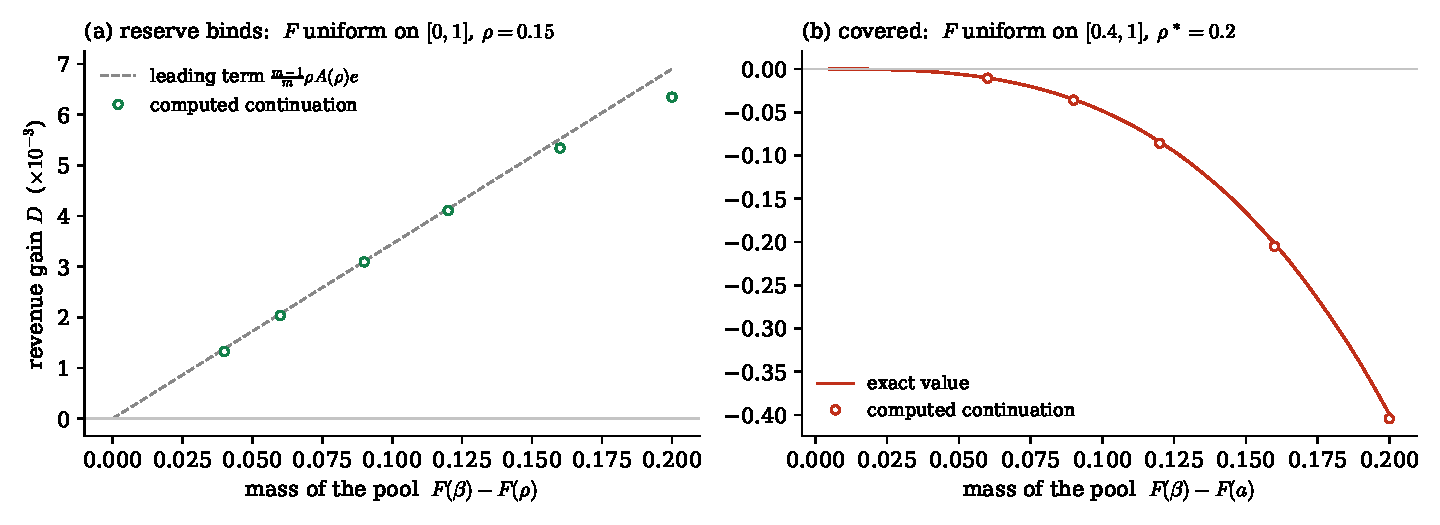
\includegraphics[width=0.86\linewidth]{figs/fig-dichotomy.pdf}

\raggedright
(a) Binding reserve ($a=0$, $\rho=0.15$): leading-order line from Theorem 3 alongside solver values. (b) Covered market ($a=0.4$, $\rho^*=0.2$): analytical curve alongside solver values (note the different vertical scales).
\end{frame}

\begin{frame}{Intuition: Why an Asking Price?}
\begin{columns}[T]
\begin{column}{0.55\textwidth}
Two forces combine when reserves bind:
\begin{itemize}
\item \alert{Net traffic capture}: buyers just above $\rho$ earn virtually zero surplus at rivals. Serving mass $e$ at price $\rho$ congests seller $1$ above the pool, costing $\frac{m+1}{2m}e$ in lost visits---leaving a \emph{net} gain of $\frac{m-1}{2m}e$ sales at $\rho$ (each earning $\rho A(\rho)^{n-1}$).
\meditem \alert{Why pooling is needed}: an efficient auction cannot hold a captured segment at reserve $\rho$---extra congestion hits the lowest types hardest, so they defect back to rivals and capture unravels from below.
\meditem<2-> \alert{Pooling stabilizes capture}: every type in $[\rho,v_1]$ gets the same flat winning probability, matching rivals' probability at the bottom.
\end{itemize}
\end{column}
\begin{column}{0.42\textwidth}
\centering\onslide<1->
\begin{tikzpicture}[scale=0.95]
  \draw[ax] (0,0)--(5.6,0) node[below,slab]{$v$};
  \draw[ax] (0,0)--(0,3.8) node[above,slab]{$\Pr(\text{win})$};
  \node[lab,below] at (0.8,0) {$\rho$};\node[lab,below] at (3.6,0) {$v_1$};
  \draw[Line,dotted] (0.8,0)--(0.8,3.5) (3.6,0)--(3.6,3.5);
  \draw[dev] (0.8,2.0)--(3.6,2.0);
  \draw[curve,dashed] plot[smooth] coordinates {(0.8,0.9) (2.2,1.9) (3.6,3.2)};
  \node[slab,anchor=west] at (3.7,3.2) {auction};
  \node[slab,text=Pool,anchor=west] at (3.7,2.0) {pool};
  \draw[Neg,-{Stealth[length=1.6mm]},line width=0.8pt] (1.2,1.25)--(1.2,1.9);
  \node[slab,text=NegDark,anchor=north west,align=left] at (1.25,1.2) {lowest types\\defect};
\end{tikzpicture}

{\scriptsize Winning probability on the captured segment $[\rho,v_1]$.}
\end{column}
\end{columns}
\end{frame}

\begin{frame}{Asymmetric Reserves Also Fail}
With $a=0$, the reserve game has no symmetric pure equilibrium (Burguet \& S\'akovics 1999), though for $m=2$, regular $F$, and large $n$ it admits an \emph{asymmetric} pure equilibrium $r_{L,n}<r_{H,n}$ with $r_{H,n}\to r_H$ solving $\psi_2(r_H)=0$ (He 2026).

\medskip
\centering
\begin{tikzpicture}[xscale=10.8]
  \node[lab,anchor=east] at (-0.02,0.21) {$L$};\node[lab,anchor=east] at (-0.02,-0.49) {$H$};
  \seg{0}{0.22}{Tint}{0}\seg{0.22}{0.5}{Dev!40}{0}\seg{0.5}{1}{Dev!15}{0}
  \seg{0}{0.4}{Tint}{-0.7}\seg{0.4}{0.5}{Card}{-0.7}\seg{0.5}{1}{Dev!15}{-0.7}
  \node[slab,text=Ink] at (0.36,0.21) {all visit $L$};\node[slab] at (0.75,0.21) {split evenly};\node[slab] at (0.75,-0.49) {split evenly};
  \node[slab] at (0.45,-0.49) {nobody};
  \foreach \x/\l in {0.22/r_L,0.4/r_H,0.5/w,1/1} \node[lab,below] at (\x,-0.72) {$\l$};
  \foreach \x in {0.22,0.4,0.5} \draw[Line,dotted] (\x,-0.7)--(\x,0.42);
\end{tikzpicture}

\raggedright\medskip\onslide<2->
\begin{block}{Theorem 4 (Asymmetric Reserves Fail for Large $n$)}
Suppose $m=2$ and $a=0$. At any sequence $(\SPA(r_{L,n}),\SPA(r_{H,n}))\to(r_L,r_H)$ with $0\le r_L<r_H<1$ and $\psi_1(r_H)<0$, for all sufficiently large $n$ seller $L$ strictly increases revenue by raising his reserve to some $v_{0,n}\in(r_{L,n},r_{H,n})$ and adding a single pool straddling the cutoff $w_n$.
\end{block}
{\footnotesize Symmetric standard-auction profiles always fail when reserves bind, and for large $n$ asymmetric duopoly profiles with $\psi_1(r_H)<0$ also fail.}
\end{frame}

%%%%%%%%%%%%%%%%%%%%%%%%%%%%%%%%%%%%%%%%%%%%%%%%%%%%%%%%%%%%%%%%%%%%
\section{Sharpness and Conclusion}
%%%%%%%%%%%%%%%%%%%%%%%%%%%%%%%%%%%%%%%%%%%%%%%%%%%%%%%%%%%%%%%%%%%%

\begin{frame}{How Sharp Is Cournot's Condition?}
In terms of demand curvature $E(v)=-\dfrac{(1-F)f'}{f^2}$, monotonicity of $\psi_m$ is $E\le m+1$. Let $\varpi(m):=\frac{m+1}{m^2+2m-1}<\frac1m$ and $\bar X:=1+\frac{1}{\varpi(m)}$.

\smallskip
\centering
\begin{tikzpicture}[xscale=1.22]
  \draw[ax] (0,0)--(10.6,0) node[right,lab]{$E(v)$};
  \fill[Pos,opacity=0.22] (0,0.02) rectangle (4.4,0.3);
  \fill[Warn,opacity=0.24] (4.4,0.02) rectangle (6.6,0.3);
  \fill[Neg,opacity=0.22] (6.6,0.02) rectangle (10.3,0.3);
  \foreach \x/\l in {2/{2},4.4/{m+1},6.6/{1+\tfrac{1}{\varpi(m)}},8.8/{2m}} {\draw[Ink,line width=0.8pt] (\x,-0.12)--(\x,0.3); \node[lab,below=2pt] at (\x,-0.1) {$\l$};}
  \draw[br] (0.03,0.44)--(1.97,0.44) node[midway,above=3pt,slab,align=center,text width=2.4cm]{regular\\(no monopoly ironing)};
  \draw[br] (2.03,0.44)--(4.37,0.44) node[midway,above=3pt,slab,align=center,text width=2.7cm]{monopoly can iron;\\no interior oligopoly pool};
  \draw[br] (4.43,0.44)--(6.57,0.44) node[midway,above=3pt,slab,align=center,text width=2.5cm]{wide pools can pay\\for large $n$};
  \draw[br] (6.63,0.44)--(10.3,0.44) node[midway,above=3pt,slab,align=center,text width=3.3cm]{narrow pools pay\\at every fixed $n$};
  \node[slab,align=center,anchor=north,text width=2.1cm] at (2,-0.78) {\textsc{Myerson}\\regularity};
  \node[slab,align=center,anchor=north,text=PosDark,text width=2.6cm] at (4.4,-0.78) {\textsc{Cournot}\\sufficient all $n$, tight $n\to\infty$};
  \node[slab,align=center,anchor=north,text width=2.3cm] at (6.6,-0.78) {Small-pool bound\\$\bar X$};
  \node[slab,align=center,anchor=north,text width=2.4cm] at (8.8,-0.78) {fixed narrow\\bands ($n\to\infty$)};
\end{tikzpicture}

\raggedright\smallskip\onslide<2->
\begin{block}{Theorem 5 (Sharpness)}
(i) For narrow pools at any fixed $n\ge 2$, the exact markup weight is $\varpi(m)<\frac1m$ (threshold $\bar X$). \quad (ii) For every $X>m+1$, some covered-market distribution with $E\le X$ admits an interior pool profitable for all large $n$, so $E\le m+1$ is tight across $n$.
\end{block}
\end{frame}

\begin{frame}{Why the Gap Opens: Small Pools vs.\ Many Buyers}
\begin{columns}[T]
\begin{column}{0.48\textwidth}
\centering
\begin{tikzpicture}[x=0.47cm,y=3.1cm]
  \draw[ax] (0.5,0)--(12.7,0) node[right,slab]{$m$};
  \draw[ax] (0.5,0)--(0.5,1.12) node[above,slab]{weight on $\frac{1-F}{f}$};
  \foreach \y in {0.2,0.4,0.6,0.8,1.0} {
    \draw[Line,line width=0.3pt] (0.35,\y)--(0.5,\y);
    \node[left,slab] at (0.32,\y) {\y};
  }
  \foreach \x in {1,2,4,6,8,10,12} {
    \draw[Line,line width=0.3pt] (\x,-0.025)--(\x,0);
    \node[below,slab] at (\x,-0.025) {\x};
  }
  \draw[InkTwo,dashed,line width=0.9pt]
    (1,1.000)--(2,0.500)--(3,0.333)--(4,0.250)--(5,0.200)--(6,0.167)
    --(7,0.143)--(8,0.125)--(9,0.111)--(10,0.100)--(11,0.091)--(12,0.083);
  \draw[Ink,line width=1.1pt]
    (1,1.000)--(2,0.429)--(3,0.286)--(4,0.217)--(5,0.176)--(6,0.149)
    --(7,0.129)--(8,0.114)--(9,0.102)--(10,0.092)--(11,0.085)--(12,0.078);
  \foreach \x/\y in {1/1.000,2/0.429,3/0.286,4/0.217,5/0.176,6/0.149,7/0.129,8/0.114,9/0.102,10/0.092,11/0.085,12/0.078}
    \fill[Ink] (\x,\y) circle (1.5pt);
  \node[slab,anchor=west] at (1.35,0.98) {Myerson ($m=1$)};
  \draw[InkTwo,dashed,line width=0.9pt] (4.8,0.82)--(6.0,0.82);
  \node[slab,anchor=west] at (6.15,0.82) {$1/m$ (Cournot)};
  \draw[Ink,line width=1.1pt] (4.8,0.66)--(6.0,0.66);
  \fill[Ink] (5.4,0.66) circle (1.5pt);
  \node[slab,anchor=west] at (6.15,0.66) {$\varpi(m)$ (small pools)};
\end{tikzpicture}

\raggedright\footnotesize
\alert{Small pools (fixed $n$)}: staircase puts $2:1$ weight on own concavity vs.\ rival cross-effect ($2\Pi_{tt}+\Pi_{tq}\le 0$), yielding $\varpi(m)<\frac1m$.
\end{column}
\begin{column}{0.48\textwidth}
\centering
\begin{tikzpicture}[scale=0.76]
  \draw[ax] (0,0)--(6.2,0) node[below,slab]{$t$};
  \draw[ax] (0,0)--(0,4.2) node[above,slab]{$\Pi(t,\uq)$};
  \draw[curve] plot[smooth,tension=0.65] coordinates {(0,0) (0.8,0.95) (1.5,1.5) (2.4,1.85) (3.3,2.25) (4.2,3.05) (5.0,3.75) (5.8,4.0)};
  \draw[InkTwo,line width=0.6pt] (0.5,0.95)--(5.9,3.4);
  \draw[dev] (1.5,1.5)--(5.0,3.75);
  \fill[Ink] (1.5,1.5) circle (1.5pt);\fill[Pool] (5.0,3.75) circle (1.5pt);
  \foreach \x/\l/\y in {1.5/\uq/1.5,5.0/\oq/3.75} {\draw[Line,dotted] (\x,0)--(\x,\y); \node[lab,below] at (\x,0) {$\l$};}
  \node[slab,anchor=north west] at (3.9,2.4) {tangent at $\uq$};
  \node[slab,text=Pool,anchor=south east] at (3.4,2.75) {secant};
\end{tikzpicture}

\raggedright\footnotesize
\alert{Many buyers ($n\to\infty$)}: $(1-q)^{n-2}$ concentrates at $\uq$; wide pools pay iff secant $>$ tangent, driving the uniform bound down to $E\le m+1$.
\end{column}
\end{columns}

\medskip\onslide<2->
\alert{From Myerson to McAfee}: for any fixed smooth $F$, interior pooling disappears once $m\ge\bar m(F)$, yet $\sup_F\bar m(F)=\infty$.
\end{frame}

\begin{frame}{Conclusion}
\begin{itemize}
\item \alert{Cournot representation}: an auctioneer's revenue under competition is a weighted integral of Cournot oligopoly revenues over market price levels, subject to Border's capacity constraint.
\meditem \alert{Covered markets}: monotonicity and nonnegativity of $\psi_m$ suffice for $\SPA(\rho^*)^m$ to survive all hierarchical deviations for every $n$, even when a monopolist would iron.
\meditem \alert{Binding reserves}: competition creates a first-order motive to misallocate: symmetric standard auctions always fail via asking prices, and for large $n$ asymmetric duopoly profiles with $\psi_1(r_H)<0$ also fail via a cutoff pool.
\meditem \alert{Sharpness}: $E\le m+1$ is tight across $n$, while $\varpi(m)<\frac1m$ is exact for narrow pools at every fixed $n$.
\end{itemize}

\onslide<2->
\begin{block}{Open questions}
\begin{enumerate}
\item What is the equilibrium when reserves bind (or when $E>\bar X$)?
\item Uniqueness of the visit continuation when multiple sellers pool simultaneously.
\item Exact finite-$n$ curvature threshold between $m+1$ and $\bar X$; mechanisms beyond $\mathcal M$ and multi-homing.
\end{enumerate}
\end{block}
\end{frame}

%%%%%%%%%%%%%%%%%%%%%%%%%%%%%%%%%%%%%%%%%%%%%%%%%%%%%%%%%%%%%%%%%%%%
\appendix
%%%%%%%%%%%%%%%%%%%%%%%%%%%%%%%%%%%%%%%%%%%%%%%%%%%%%%%%%%%%%%%%%%%%

\begin{frame}[noframenumbering]{Backup: Related Literature}
\begin{itemize}
\item \alert{Monopoly auctions}: Myerson (1981), Bulow \& Roberts (1989).
\meditem \alert{Large-market competing auctions}: McAfee (1993), Peters (1997), Peters \& Severinov (1997), Hernando-Veciana (2005), Ma \& Riquelme (2026).
\meditem \alert{Finite-market reserve competition}: Burguet \& S\'akovics (1999), Vir\'ag (2007, 2010), He (2026).
\meditem \alert{Directed search \& asking prices}: Burdett, Shi \& Wright (2001), Eeckhout \& Kircher (2010), Albrecht, Gautier \& Vroman (2014), Lester, Visschers \& Wolthoff (2017), Wright et al.\ (2021).
\meditem \alert{Competitive screening \& redistributive design}: Armstrong \& Vickers (2001), Rochet \& Stole (2002), Stole (2007), Chade \& Swinkels (2021), Dworczak, Kominers \& Akbarpour (2021).
\meditem \alert{Methods}: Border (1991), Che, Kim \& Mierendorff (2013), Kleiner, Moldovanu \& Strack (2021), Monderer \& Shapley (1996).
\end{itemize}
\end{frame}

\begin{frame}[noframenumbering]{Backup: Potential Game Details (Proposition 1)}
\begin{itemize}
\item In a second price auction, a visitor's realized surplus equals her marginal contribution to reserve-truncated welfare $\widetilde W_j(S_j)=(\max_{k\in S_j}v_k-r_j)^+$.
\meditem Hence the visit subgame is an exact potential game (Monderer \& Shapley 1996) with concave potential $\Phi(\theta)=\sum_j\int_{r_j}^1[1-F_j(v)^n]\,dv$.
\meditem Directional derivative in $\tilde\theta-\theta$ equals $n\sum_j\int_a^1(\tilde\theta_j-\theta_j)s_j f\,dv$, so stationarity is equivalent to sequential rationality.
\meditem When seller $1$ posts $r_1\ge\rho$ against rivals at $\rho$, the cutoff $w\in[r_1,1]$ uniquely solves
\[
(w-r_1)\,A(w)^{n-1} = \int_\rho^w F_{\mathrm{riv}}(v;w)^{n-1}\,dv, \qquad F_{\mathrm{riv}}(v;w):=A(w)-\frac{F(w)-F(v)}{m-1}.
\]
\end{itemize}
\end{frame}

\begin{frame}[noframenumbering]{Backup: Uniqueness Across a Pool (Proposition 2)}
On a pool $(\alpha_i,\beta_i)$, $\bar x_i=g(F_1(\alpha_i),F_1(\beta_i))$ is strictly increasing in both endpoints.
\begin{block}{Key Step}
If $(\Delta F,\Delta\sigma)$ is positive ($\Delta F>0,\Delta\sigma\ge 0$) at $\alpha_i$, then at $\beta_i$ it is either strictly positive or strictly negative---never $(0,0)$.
\end{block}
\begin{itemize}
\item If $\Delta\bar x_i\ge 0$: $\Delta\sigma'=\Delta\bar x_i+(x_{\mathrm{riv}}-\tilde x_{\mathrm{riv}})\ge 0$ while $\Delta F>0$, keeping the pair strictly positive to $\beta_i$.
\item If $\Delta\bar x_i<0$: then $\Delta F(\beta_i)<0$; past the last zero $z_0$ of $\Delta F$, $\Delta\sigma'<0$, forcing $\Delta\sigma<0$ at $\beta_i$.
\end{itemize}

\medskip
\centering
\begin{tikzpicture}[xscale=10.6]
  \seg{0}{0.2}{Card}{0}\seg{0.2}{0.38}{Pool!55}{0}\seg{0.38}{0.6}{Card}{0}\seg{0.6}{0.75}{Pool!55}{0}\seg{0.75}{1}{Card}{0}
  \node[slab] at (0.29,0.21) {pool};\node[slab] at (0.675,0.21) {pool};
  \node[slab] at (0.1,0.21) {sign kept};\node[slab] at (0.49,0.21) {sign kept};\node[slab] at (0.875,0.21) {sign kept};
  \node[slab,text=Pool,above] at (0.29,0.42) {may flip};\node[slab,text=Pool,above] at (0.675,0.42) {may flip};
  \node[lab,below] at (0,-0.02) {$\underline r$};\node[lab,below] at (1,-0.02) {$1$};
  \node[slab,text=NegDark,anchor=west] at (1.01,0.21) {$\Delta F(1)\neq0$};
\end{tikzpicture}
\end{frame}

\begin{frame}[noframenumbering]{Backup: Band Structure Numerics (Lemma 1)}
\begin{columns}[T]
\begin{column}{0.48\textwidth}
\begin{itemize}
\item On the pool, seller $1$'s allocation is flat. Indifference requires rivals' effective distribution to be flat too, so rivals get \emph{no} traffic on $(v_2,v_3)$.
\meditem Types near $\alpha$ lose from pooling and leave; types just above $\beta$ have a temporary surplus deficit and also leave.
\meditem Pool endpoints are exact $F_{\mathrm{riv}}^{n-1}$-averages of $v$ on the two outer sub-bands:
\[
\alpha = \frac{\int_{v_1}^{v_2}v\,dF_{\mathrm{riv}}^{n-1}}{\int_{v_1}^{v_2}dF_{\mathrm{riv}}^{n-1}},\quad
\beta = \frac{\int_{v_3}^{v_4}v\,dF_{\mathrm{riv}}^{n-1}}{\int_{v_3}^{v_4}dF_{\mathrm{riv}}^{n-1}}.
\]
\end{itemize}
\end{column}
\begin{column}{0.49\textwidth}
\centering
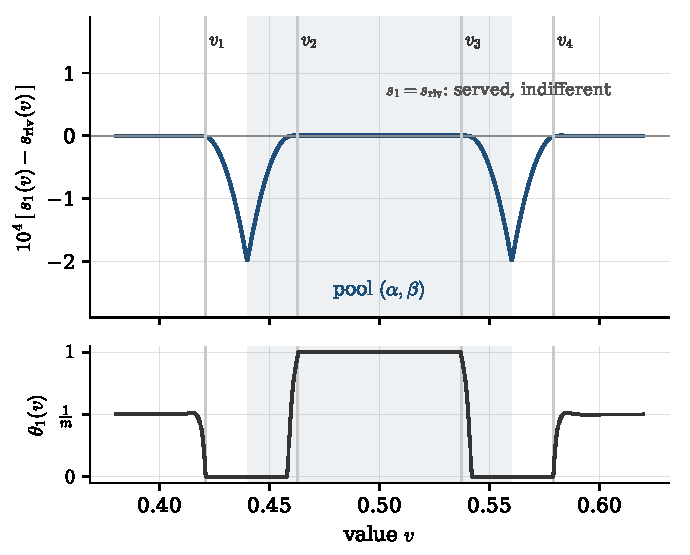
\includegraphics[width=\linewidth]{figs/fig-band.pdf}

{\scriptsize Uniform $F$, $m=n=2$, pool $(0.44,0.56)$. Predicted band points $(0.42,0.46,0.54,0.58)$ match the equilibrium solver.}
\end{column}
\end{columns}
\end{frame}

\begin{frame}[noframenumbering]{Backup: A Smaller Seller Does Not Pool (Corollary 1)}
\begin{columns}[T]
\begin{column}{0.54\textwidth}
\begin{block}{Corollary 1}
Suppose rivals post $\SPA(\rho)$ (binding or not) and $\psi_m$ is nondecreasing on $[\max\{\rho,a\},1]$. Any deviation leaving seller $1$'s customers indifferent and $t_0\le q_0$ earns at most the standard auction $\SPA(r)$ ($r\ge\rho$) inducing traffic $t_0$.
\end{block}
\smallskip
Intuitively, the deviator faces the truncated inverse demand curve $\max\{P(z),\rho\}$, which is flat at the rivals' reserve. Two ways to gain: stay small (where $\SPA$ dominates) or flood the flat bottom.
\end{column}
\begin{column}{0.43\textwidth}
\centering
\begin{tikzpicture}[scale=0.84]
  \draw[ax] (0,0)--(6.2,0) node[below left,slab]{total quantity $z$};
  \draw[ax] (0,0)--(0,4.1) node[above,slab]{price};
  \draw[Line,dashed] plot[smooth] coordinates {(3.4,1.5) (4.4,0.8) (5.4,0.25)};
  \draw[curve] plot[smooth] coordinates {(0,3.9) (1,3.2) (2,2.5) (3,1.8) (3.4,1.5)};
  \draw[curve] (3.4,1.5)--(5.9,1.5);
  \node[slab,left] at (0,1.5) {$\rho$};
  \draw[Line,dotted] (0,1.5)--(3.4,1.5);
  \node[slab,anchor=south west] at (1.2,3.1) {$\max\{P(z),\rho\}$};
  \draw[dev,-{Stealth[length=1.6mm]}] (2.6,0.5)--(1.6,0.5) node[midway,below,slab,text=Pool]{stay small};
  \draw[dev,-{Stealth[length=1.6mm]}] (4.0,0.5)--(5.4,0.5) node[midway,below,slab,text=Pool]{flood};
\end{tikzpicture}
\end{column}
\end{columns}
\end{frame}

\begin{frame}[noframenumbering]{Backup: Asymmetric Reserves Details (Theorem 4)}
\centering
\begin{tikzpicture}[xscale=10.8]
  \node[lab,anchor=east] at (-0.02,0.21) {before};\node[lab,anchor=east] at (-0.02,-0.69) {after};
  \seg{0}{0.18}{Tint}{0}\seg{0.18}{0.52}{Dev!40}{0}\seg{0.52}{1}{Dev!15}{0}
  \seg{0}{0.31}{Tint}{-0.9}\seg{0.31}{0.44}{Dev!40}{-0.9}\seg{0.44}{0.64}{Pool!55}{-0.9}\seg{0.64}{0.72}{Riv}{-0.9}\seg{0.72}{1}{Dev!15}{-0.9}
  \node[slab,text=Ink] at (0.35,0.21) {all visit $L$};\node[slab] at (0.76,0.21) {split evenly};
  \node[slab,text=Ink] at (0.375,-0.69) {$L$ only};\node[slab] at (0.54,-0.69) {pool, $L$ only};\node[slab] at (0.68,-0.69) {$H$};\node[slab] at (0.86,-0.69) {split evenly};
  \foreach \x/\l in {0.18/r_L,0.4/r_H,0.52/w} \node[lab,above] at (\x,0.42) {$\l$};
  \foreach \x in {0.4,0.52} \draw[Line,dotted] (\x,0.42)--(\x,-0.9);
  \node[slab,anchor=north] at (0.31,-0.92) {new reserve $v_{0,n}$};
\end{tikzpicture}

\raggedright\smallskip
\begin{itemize}
\item \alert{Low-reserve seller $L$}: raises reserve to $v_{0,n}\in(r_{L,n},r_{H,n})$ and pools width $O(1/n)$ (scaled by $u>0$) across $w_n$. As $n\to\infty$, the rescaled gain converges to
\[
\lim_{n\to\infty} \frac{D_n}{(1-q_{w_n})^n} \;=\; -\frac{u^2}{6}\,\psi_1(r_H) + O(u^4) \;>\; 0
\]
for small $u>0$ whenever $\psi_1(r_H)<0$. At He's (2026) reserve ($\psi_2(r_H)=0$), the exact limit simplifies identically to $r_H\bigl(\frac{\sinh u}{u}-1\bigr) > 0$.
\meditem \alert{High-reserve seller $H$}: by Corollary 1, cannot gain while staying smaller than $L$ ($t_0\le q_0$).
\end{itemize}
\end{frame}

\begin{frame}[noframenumbering]{Backup: Many Buyers: Weight Concentration (Proposition C.2)}
\begin{columns}[T]
\begin{column}{0.54\textwidth}
As $n\to\infty$, $(1-q)^{n-2}$ concentrates at $\uq$ while the jump $q^*-\uq\approx\frac{\log n}{n}\to 0$:
\begin{itemize}
\item For any fixed interior band $[\uq,\oq]$,
\[
\lim_{n\to\infty}\frac{D_n}{(1-\uq)^n} = \frac{\Pi(\oq,\uq)-\Pi(\uq,\uq)}{\oq-\uq} - \partial_t\Pi(\uq,\uq).
\]
\meditem \alert{Non-commuting limits}: taking $d\to 0$ first at fixed $n$ gives $\bar X=1+\frac{1}{\varpi(m)}$, whereas taking $n\to\infty$ first on a fixed narrow band gives $E\le 2m$.
\meditem \alert{Wide bands}: comparing secant to tangent near the top of the market drives the uniform bound down to Cournot's $E\le m+1$.
\end{itemize}
\end{column}
\begin{column}{0.45\textwidth}
\centering
\begin{tikzpicture}[scale=3.5]
  \draw[ax] (0,0)--(1.1,0) node[below,slab]{$q$};
  \draw[ax] (0,0)--(0,1.1) node[above,slab]{$t$};
  \draw[Line,dashed] (0,0)--(1,1);
  \draw[dev] (0.25,0.25)--(0.34,0.25)--(0.34,0.85)--(0.85,0.85);
  \draw[curve,InkTwo,domain=0.25:0.95,samples=60] plot (\x,{0.6*exp(-14*(\x-0.25))});
  \node[slab,anchor=west] at (0.4,0.12) {weight $(1-q)^{n-2}$};
  \foreach \x/\l in {0.25/\uq,0.34/q^*,0.85/\oq} \node[lab,below] at (\x,0) {$\l$};
\end{tikzpicture}
\end{column}
\end{columns}
\end{frame}

\end{document}
